\documentclass[a4paper,11pt]{article}

\usepackage[T1]{fontenc}
\usepackage[utf8]{inputenc}
\usepackage{float}
\usepackage{xcolor}
\usepackage{parskip}
\usepackage{tgtermes}
\usepackage{graphicx,wrapfig}
\usepackage[
pdftitle={Math Assignment}, 
pdfauthor={Lucas Varela, Universidad de los Andes},
colorlinks=true,linkcolor=blue,urlcolor=blue,citecolor=blue,bookmarks=true,
bookmarksopenlevel=2]{hyperref}
\usepackage{amsmath,amssymb,amsthm,textcomp}
\usepackage{enumerate}
\usepackage{multicol}
\usepackage{tikz}
\definecolor{pr}{HTML}{FF6961}
\definecolor{pb}{HTML}{779ecb}
\usepackage{hyperref}

\definecolor{pg}{HTML}{77DD77}

\usepackage{geometry}
\geometry{total={210mm,297mm},
	left=25mm,right=25mm,%
	bindingoffset=0mm, top=20mm,bottom=20mm}


\linespread{0.9}

\newcommand{\linia}{\rule{\linewidth}{0.5pt}}

% custom theorems if needed


% my own titles
\makeatletter
\renewcommand{\maketitle}{
	\begin{center}
		\vspace{2ex}
		{\huge \textsc{\@title}}
		\vspace{1ex}
		\\
		\linia\\
		\@author \hfill \@date
		\vspace{4ex}
	\end{center}
}
\makeatother
%%%

% custom footers and headers
\usepackage{fancyhdr,lastpage}
\pagestyle{fancy}
\lhead{}
\chead{}
\rhead{}
\lfoot{}
\cfoot{}
\rfoot{Page \thepage\ /\ \pageref*{LastPage}}
\renewcommand{\headrulewidth}{0pt}
\renewcommand{\footrulewidth}{0pt}
%

%%%----------%%%----------%%%----------%%%----------%%%

\begin{document}
	\title{Movimiento Relativo}
	
	\author{Física I}
	
	\date{}
	
	\maketitle
	
			
\tableofcontents

	\section{Velocidad relativa}
	
	La forma más fácil de entender la velocidad relativa es con vectores. Considere un observador \textbf{a} y otro observador \textbf{b}. Estos dos observadores están a una distancia $\vec{\textbf{s}}_{\textbf{a}}$, medida desde el marco de referencia de \textbf{a}. Ahora piense que hay un objeto $m$. Este objeto $m$ esta a una distancia $\vec{\textbf{r}}_{\textbf{b}}$ del observador \textbf{b}. Ahora quisiéramos ver la posición a la que se encuentra $m$, medido desde el marco \textbf{a}. Esta posición la llamamos $\vec{\textbf{r}}_{\textbf{a}}$ y se obtiene a partir de $\vec{\textbf{s}}_{\textbf{a}}$ y $\vec{\textbf{r}}_{\textbf{b}}$ con la siguiente relación:
	
	
	\begin{equation}\label{1}
	\vec{\textbf{r}}_{\textbf{a}} = \vec{\textbf{s}}_{\textbf{a}} + \vec{\textbf{r}}_{\textbf{b}}
	\end{equation}
	
	
	La situación se muestra en el siguiente dibujo:
	
	\begin{figure}[h]
		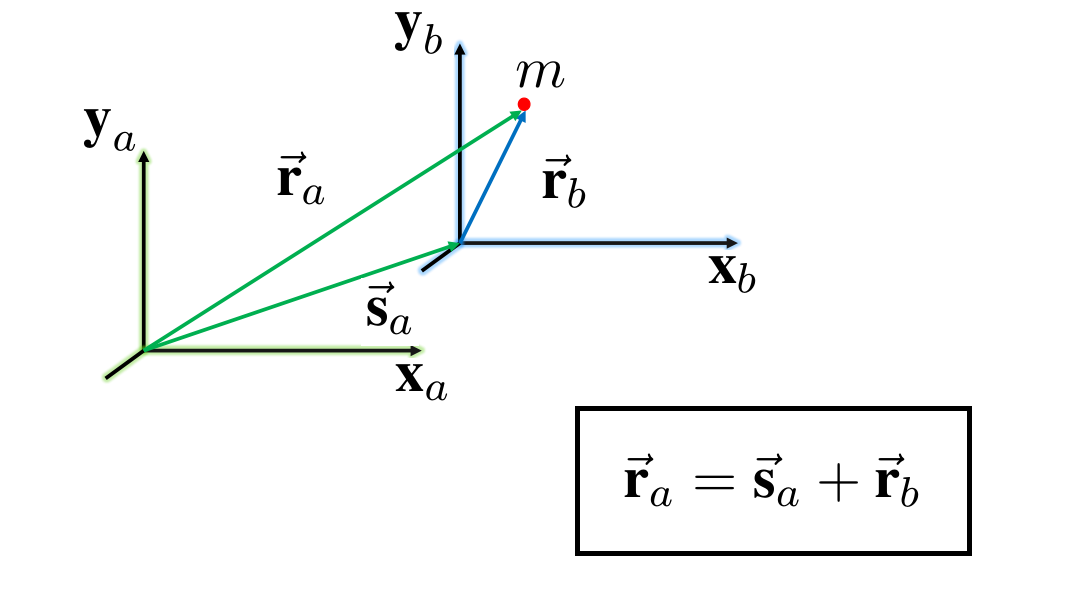
\includegraphics[width=.9\linewidth]{./im/mvtorela}
		\label{fcN4}
	\end{figure}
	
	
	Si el objeto $m$ y el observador \textbf{b} se están moviendo, quisiéramos saber que relación hay entre las velocidades que mide el observador \textbf{a} y el observador \textbf{b}. Para ello se deriva la relación \ref{1} con respecto al tiempo y se obtienen la relación de las velocidades:
	
	\begin{equation}\label{2}
	\vec{\textbf{v}}_{\textbf{a}} = \vec{\textbf{v}}_{\textbf{R}_\textbf{a}} + \vec{\textbf{v}}_{\textbf{b}}
	\end{equation}
	
	En la igualdad anterior reconocemos las siguientes cantidades:
	
	\begin{itemize}
		\item $\vec{\textbf{v}}_{\textbf{a}}$: Velocidad del objeto $m$ vista por el observador \textbf{a} (con respecto al observador \textbf{a})
		\item $\vec{\textbf{v}}_{\textbf{b}}$: Velocidad del objeto $m$ vista por el observador \textbf{b} (con respecto al observador \textbf{b})
		\item $\vec{\textbf{v}}_{\textbf{R}_\textbf{a}}$: Velocidad del observador \textbf{b} vista por el observador \textbf{a}(velocidad relativa entre el observador \textbf{b} y el \textbf{a})
	\end{itemize}
	
	\section{Ejemplos}
	
		\color{pb}
	\subsection{Anacleta \& Bartolomeo I}
	
	\textbf{Anacleta conduce su carro a 100km/h con respecto a la tierra. Anacleta ve pasar a Bartolomeo en la misma dirección  a 30km/h. ¿Cuál es la velocidad de Bartolomeo con respecto a la tierra?}\\	\color{black}
	
	
	
	Primero identifiquemos que información tenemos y cual queremos obtener. Se tiene la velocidad de Anacleta con respecto a la tierra. Se tiene la velocidad de Bartolomeo con respecto a Anacleta y se quiere saber la velocidad de Bartolomeo con respecto a la tierra. Identifiquemos nuestro observador \textbf{a} es la tierra. El observador \textbf{b} es Anacleta y el objeto $m$ es Bartolomeo. Ahora la velocidad que se conocen son:
	
	
	\begin{figure}[h]
		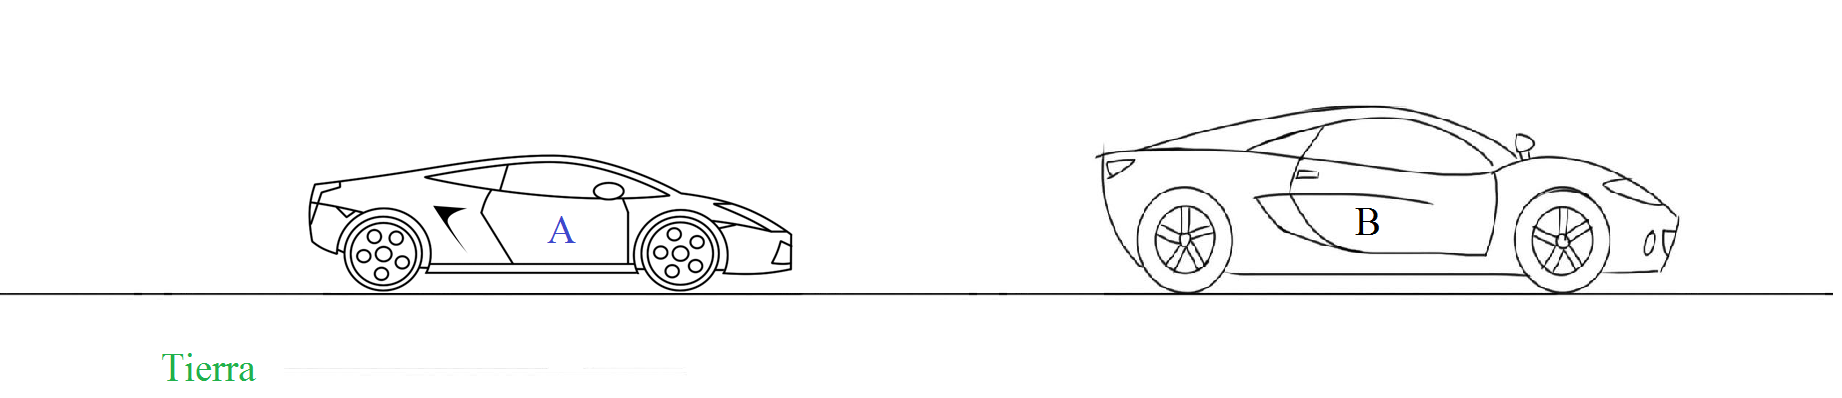
\includegraphics[width=.9\linewidth]{./im/c2}
		\label{fcN4}
		\caption{Imagenes tomadas de [1]}
	\end{figure}
	
	
	$$ \vec{\textbf{v}}_{\textbf{s}_\textbf{a}} = 100 \text{ km/h } \boldsymbol{\hat{\imath}} $$
	$$ \vec{\textbf{v}}_{\textbf{b}} = 20 \text{ km/h } \boldsymbol{\hat{\imath}}$$ 
	
	
	Utilizando la relación \ref{2} se obtiene la velocidad $\vec{\textbf{v}}_{\textbf{a}}$ (la velocidad de Bartolomeo medida desde la tierra):
	
	\begin{equation}
	\vec{\textbf{v}}_{\textbf{a}} = \vec{\textbf{v}}_{\textbf{R}_\textbf{a}} + \vec{\textbf{v}}_{\textbf{b}} = 100 \text{ km/h }\boldsymbol{\hat{\imath}} + 20 \text{ km/h } \boldsymbol{\hat{\imath}}
	\end{equation}
	
	Por lo que la velocidad de Bartolomeo medida desde la tierra es:
	
	\begin{equation}
	\vec{\textbf{v}}_{\textbf{a}}= 120 \text{ km/h } \boldsymbol{\hat{\imath}}
	\end{equation}
		\color{pb}
		\subsection{Anacleta \& Bartolomeo II}
	
	\textbf{Anacleta conduce su carro a 100km/h con respecto a la tierra. Anacleta ve pasar a Bartolomeo en la dirección opuesta a 30km/h. ¿Cuál es la velocidad de Bartolomeo con respecto a la tierra?\\}	\color{black}
	
	Lo único que cambia en este problema es que ahora la velocidad $\vec{\textbf{v}}_{\textbf{b}}$ tiene el signo opuesto, ya que Bartolomeo ahora se mueve en la dirección opuesta a el observador \textbf{b}, Anacleta. Entonces se tiene:
	
	
	$$ \vec{\textbf{v}}_{\textbf{R}_\textbf{a}} = 100 \text{ km/h } \boldsymbol{\hat{\imath}} $$
	$$ \vec{\textbf{v}}_{\textbf{b}} = -20 \text{ km/h } \boldsymbol{\hat{\imath}}$$ 
	
	Por lo que usando la ecuación \ref{2}:
	\begin{equation}
	\vec{\textbf{v}}_{\textbf{a}} = \vec{\textbf{v}}_{\textbf{R}_\textbf{a}} + \vec{\textbf{v}}_{\textbf{b}} = 100 \text{ km/h }\boldsymbol{\hat{\imath}} - 20 \text{ km/h } \boldsymbol{\hat{\imath}}
	\end{equation}
	
	Obteniendo asi, que la velocidad de Bartolomeo con respecto a la tierra es:
	
	\begin{equation}
	\vec{\textbf{v}}_{\textbf{a}}= 80 \text{ km/h } \boldsymbol{\hat{\imath}}
	\end{equation}
	
	
	Note que en ambos casos Bartolomeo se mueve en la misma dirección \textbf{con respecto a la tierra}. Sin embargo la magnitud de su velocidad no es la misma para ambos casos.
		\color{pb}
	\subsection{Mythbusters}
	\textbf{En el episodio 140(``Spy car scape'') del programa Mythbusters se hizo un experimento de velocidad relativa. El experimento consiste en lo siguiente. Considere un carro que se mueve con una velocidad de -60 mi/h con respecto a una cámara en el piso. Desde el carro se dispara un balón de fútbol a 60 mi/h con respecto al carro. ¿Qué velocidad tiene el balón con respecto a la cámara y cómo sera la trayectoria del balón que ve la cámara?
		\\ }	\color{black}
	
	Se identifica la cámara como el observador \textbf{a}, el carro como el observador \textbf{b} y el balón como el objeto. Las velocidades que conocemos son:
	
	
	$$ \vec{\textbf{v}}_{\textbf{R}_\textbf{a}} = -60 \text{ mi/h } \boldsymbol{\hat{\imath}} $$
	$$ \vec{\textbf{v}}_{\textbf{b}} = 60 \text{ mi/h } \boldsymbol{\hat{\imath}}$$ 
	
	Ahora usando la ecuación \ref{2}:
	\begin{equation}
	\vec{\textbf{v}}_{\textbf{a}} = \vec{\textbf{v}}_{\textbf{R}_\textbf{a}} + \vec{\textbf{v}}_{\textbf{b}} = -60 \text{ mi/h }\boldsymbol{\hat{\imath}} + 60 \text{ mi/h } \boldsymbol{\hat{\imath}}
	\end{equation}
	
	Por lo tanto la velocidad del balón visto por la cámara es $0 $mi/h. Es decir no tiene velocidad en la dirección horizontal. Como el cañon que lo dispara esta elevado tiene una altura inicial. Como no hay velocidad en $x$ este tiene un movimiento de caída libre. En el siguiente vídeo se puede ver como cae el balón con dirección completamente vertical: \url{https://www.youtube.com/watch?v=qQVDAMzo4mE}
	
		\color{pb}
	\subsection{Anacleta \& Bartolomeo III}
	\textbf{Anacleta y Bartolomeo deciden irse de paseo en carro a coveñas. Anacleta que es más madrugadora sale primero conduce su carro a $\frac{1}{36}$km/s. Faltando $20$ km para llegar a coveñas, Anacleta ve pasar a Bartolomeo. Anacleta tiene una muy buena visión y puede ver hasta un 1 km de distancia. Luego de 20 s de que Bartolomeo le pasara por el lado ya no puede verlo. ¿Cuál es la velocidad de Bartolomeo con respecto a la tierra? Asuma que ambos viajan a velocidad constante.\\
	}	\color{black}
	
	En el momento que Anacleta para de ver Bartolomeo el está a 1 km de ella. Bartolomeo tardo 20 s en recorrer 1km respecto a Anacleta. Por lo tanto la velocidad de Bartolomeo respecto a Anacleta es:
	
	$$ \vec{\textbf{v}}_{\textbf{b}} = 1/20 \text{ km/s } \boldsymbol{\hat{\imath}}$$ 
	
	
	La velocidad de Anacleta respecto a la tierra es $  \vec{\textbf{v}}_{\textbf{R}_\textbf{a}}=\frac{1}{36}$ km/s, por lo que usando la relación \ref{2} se obtiene $ \vec{\textbf{v}}_{\textbf{a}}$:
	
	\begin{equation}
	\vec{\textbf{v}}_{\textbf{a}} = \vec{\textbf{v}}_{\textbf{R}_\textbf{a}} + \vec{\textbf{v}}_{\textbf{b}} =  \frac{1}{36}\text{ km/s }\boldsymbol{\hat{\imath}} + \frac{1}{20} \text{ km/s } \boldsymbol{\hat{\imath}}
	\end{equation}
	
	Entonces la velocidad de Bartolomeo respecto a la tierra es:
	
	
	\begin{equation}
	\vec{\textbf{v}}_{\textbf{a}} = \frac{7}{90} \text{ km/s } \boldsymbol{\hat{\imath}} = 280 \text{ km/h}
	\end{equation}
	
		\color{pb}
	\subsection{Tenis}
	\textbf{Una pelota de tenis rebota contra una raqueta. Luego del impacto la velocidad de la raqueta no cambia. Además, la velocidad relativa entre la pelota y la raqueta solo cambia su dirección pero tiene la misma magnitud. Suponga que desde el marco de referencia de un espectador la raqueta se mueve hacia la pelota con una rapidez de 10 m/s. La pelota desde el marco del espectador se mueve con rapidez 20 m/s hacia la raqueta. ¿Con qué velocidad, relativa al espectador saldrá la pelota luego de rebotar con la raqueta?\\
	} 
		\color{black}
	
	El enunciado nos dice que si sabemos la velocidad relativa entre la pelota y la raqueta antes del impacto, sabemos también la velocidad relativa entre la pelota y la raqueta después del impacto. Encontremos primero la velocidad relativa entre la pelota y la raqueta antes del impacto. Entonces nuestro observador \textbf{a}  en este caso es el espectador. El  observador \textbf{b} es la raqueta y el objeto $m$ es la pelota. La siguiente imagen representa la situación vista por el espectador.
	
	
	
	
	\begin{figure}[h]
		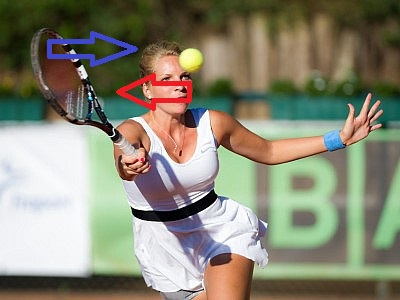
\includegraphics[width=1.0\linewidth]{./im/ten}
		\caption{Situación antes del impacto. Imagen saca de [2]}
	\end{figure}
	
	
	
	Donde conocemos las siguientes cantidades:
	
	
	
	
	$$ \vec{\textbf{v}}_{\textbf{R}_\textbf{a}} = 10 \text{ m/s } \boldsymbol{\hat{\imath}} \qquad \text{Velocidad de la raqueta relativa al espectador}$$
	$$ \vec{\textbf{v}}_{\textbf{a}} = -20 \text{ m/s } \boldsymbol{\hat{\imath}} \qquad \text{Velocidad de la pelota relativa al espectador}$$ 
	
	Por lo tanto utilizando la relación \ref{2} se tiene:
	
	
	\begin{equation}
	\vec{\textbf{v}}_{\textbf{a}} = \vec{\textbf{v}}_{\textbf{R}_\textbf{a}} + \vec{\textbf{v}}_{\textbf{b}} 
	\end{equation}
	
	
	\begin{equation}
	-20 \text{ m/s } \boldsymbol{\hat{\imath}} =  10 \text{ m/s } \boldsymbol{\hat{\imath}} + \vec{\textbf{v}}_{\textbf{b}} 
	\end{equation}
	
	\begin{equation}
	\vec{\textbf{v}}_{\textbf{b}}=  -30 \text{ m/s } \boldsymbol{\hat{\imath}}  
	\end{equation}
	
	Recuerde que  $\vec{\textbf{v}}_{\textbf{b}} = -30  \text{ m/s } \boldsymbol{\hat{\imath}} $, corresponde  la velocidad de la pelota relativa a la raqueta antes del impacto.
	
	
	
	
	 \textbf{Ahora analicemos la situación luego del impacto:} 
	
	
	\begin{figure}[h]
		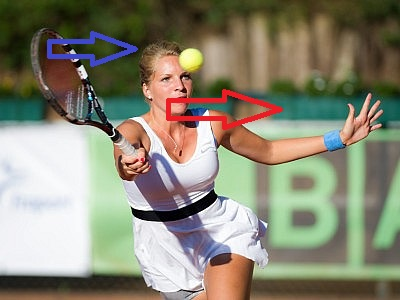
\includegraphics[width=1.0\linewidth]{./im/ten2}
		\caption{Situación después del impacto. Imagen saca de [2]}
	\end{figure}
	
	El enunciado nos dice que ahora la velocidad de la pelota relativa a la raqueta cambia su dirección pero no su magnitud, es decir que:
	
	$$\vec{\textbf{v}}_{\textbf{b}} = 30  \text{ m/s } \boldsymbol{\hat{\imath}} $$
	
	El enunciado nos dice que además la raqueta mantiene su velocidad relativa al espectador igual, es decir que $\vec{\textbf{v}}_{\textbf{R}_\textbf{a}}$ sigue siendo:
	
	$$ \vec{\textbf{v}}_{\textbf{R}_\textbf{a}} = 10 \text{ m/s } \boldsymbol{\hat{\imath}} $$
	
	Usando nuevamente la relación \ref{2} pero con estos nuevos valores se obtiene:
	
	
	
	\begin{equation}
	\vec{\textbf{v}}_{\textbf{a}} = \vec{\textbf{v}}_{\textbf{R}_\textbf{a}} + \vec{\textbf{v}}_{\textbf{b}} = 10 \text{ m/s } \boldsymbol{\hat{\imath}} + 30 \text{ m/s } \boldsymbol{\hat{\imath}}
	\end{equation}
	
	Por lo que la velocidad final de la pelota relativa al espectador $\vec{\textbf{v}}_{\textbf{a}}$ es:
	
	\begin{equation}
	\vec{\textbf{v}}_{\textbf{a}} =  40 \text{ m/s } \boldsymbol{\hat{\imath}} 
	\end{equation}
	
	\color{pb}
	\subsection{Aves migratorias (Movimiento relativo en 2D)}
	
	\textbf{Los gansos canadienses viajan principalmente en dirección norte-sur por mucho más de mil kilómetros en
		algunos casos, viajando a velocidades hasta de 100 km/h aproximadamente. Si una de estas aves vuela a 100 km/h en relación con el aire,pero hay un viento de 40 km/h que sopla de oeste a este, a) ¿a qué
		ángulo en relación con la dirección norte-sur debería volar esta ave
		de modo que viaje directamente hacia el sur en relación con el suelo?
		b) ¿Cuánto tiempo le tomará al ganso cubrir una distancia terrestre de
		500 km de norte a sur? (Nota: Incluso en noches nubladas, muchas
		aves pueden volar usando el campo magnético de la Tierra para identificar la dirección norte-sur).\\}
	\color{black}
	
	Primero que todo, identifiquemos nuestros observadores y objeto. El observador \textbf{a} es la tierra. El observador \textbf{b} es el aire y el observador objeto $m$ es el ganso canadiense. Nos dicen la velocidad relativa del aire con respecto a la tierra es de 40km/h de oeste a este(tomaremos esta como la dirección $\boldsymbol{\hat{\imath}}$. Nos dan solo la rapidez del ganso respecto al aire, pero no la dirección. Por último nos preguntan que dirección debe tener para que la velocidad de ganso respecto a la tierra sea solo en la dirección Norte-Sur(tomaremos esta dirección como $-\boldsymbol{\hat{\jmath}}$).  $\theta$ 
	
	
	
	
	
	\begin{figure}[h]
		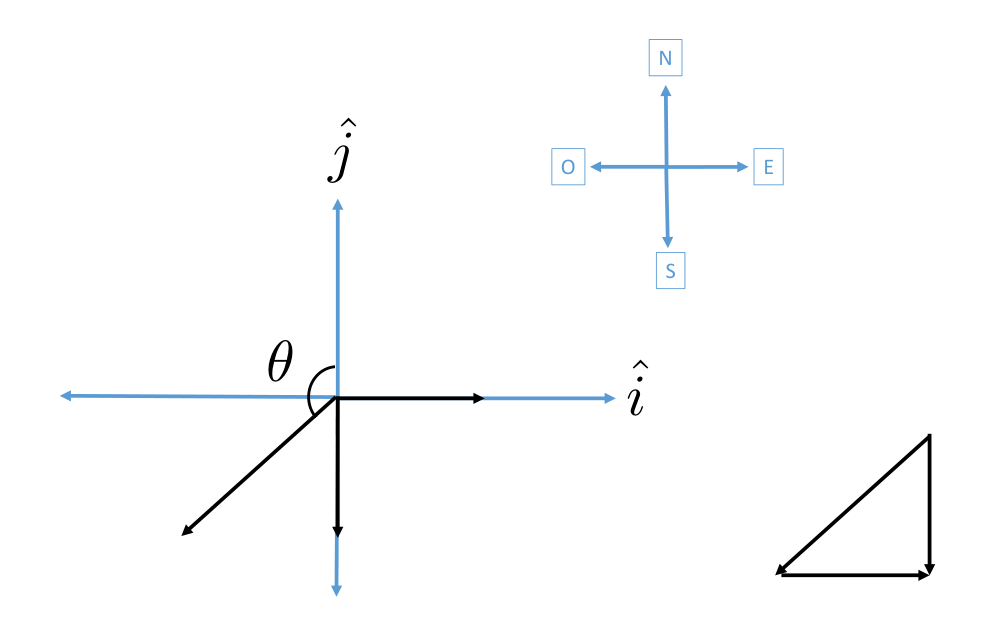
\includegraphics[width=1.0\linewidth]{./im/4}
	\end{figure}
	
	Las velocidades son:
	
	$$   \vec{\textbf{v}}_{\textbf{b}}  = -100 \sin (180-\theta \boldsymbol{\hat{\imath}}) + 100\cos (180-\theta) \boldsymbol{\hat{\jmath}} $$
	
	$$ \vec{\textbf{v}}_{\textbf{R}_\textbf{a}}  = 40\; \boldsymbol{\hat{\imath}} + 0\; \boldsymbol{\hat{\jmath}}  $$
	
	$$ \vec{\textbf{v}}_{\textbf{a}} = 0\; \boldsymbol{\hat{\imath}} -\textbf{v}_{\textbf{a}} \; \boldsymbol{\hat{\jmath}}   $$
	
	Donde se puso $(180-\theta)$ para usar el ángulo que forma la velocidad medido de Sur hacia Oeste(en sentido horario). Ahora, la relación \ref{2} nos dice que:
	
	
	
	$$
	\vec{\textbf{v}}_{\textbf{a}} = \vec{\textbf{v}}_{\textbf{R}_\textbf{a}} + \vec{\textbf{v}}_{\textbf{b}}$$
	
	
	Que en este caso es:
	
	
	$$
	0\; \boldsymbol{\hat{\imath}}-{v}_{\textbf{a}} \; \boldsymbol{\hat{\jmath}}  = (40\; \boldsymbol{\hat{\imath}}+ 0\; \boldsymbol{\hat{\jmath}} ) + (-100 \sin(180-\theta) \boldsymbol{\hat{\imath}} + 100\cos(180-\theta) \boldsymbol{\hat{\jmath}})   
	$$
	
	
	Esto se puede simplificar agrupando los términos en cada dirección:
	
	
	\begin{equation}
	0\; \boldsymbol{\hat{\imath}}-{v}_{\textbf{a}} \; \boldsymbol{\hat{\jmath}}  = (40 -100 \sin \theta)\; \boldsymbol{\hat{\imath}} + 100\cos \theta \boldsymbol{\hat{\jmath}}   
	\end{equation}
	
	De esta igualdad vectorial se sacan 2 igualdades, una por cada componente:
	
	\begin{equation}\label{be1}
	0 = 40 -100 \sin (180-\theta)
	\end{equation}
	
	\begin{equation}\label{be2}
	-v_{\textbf{a}} = 100\cos (180-\theta)
	\end{equation}
	
	De la igualdad \ref{be1} obtenemos el ángulo $\theta$
	
	$$  \sin (180-\theta) = 4/10 $$ 
	
	$$   180-\theta = 23.58 $$ 
	
	
	Entonces $\theta= 156.42 $. Ahora piden encontrar cuanto se demora el ganso en estas condiciones en recorrer 500 km de norte a sur. Para ello se obtiene la velocidad relativa del ganso con respecto a la tierra  $\vec{\textbf{v}}_{\textbf{a}}$, lo cual podemos hallar de la relación \ref{be2} y con el ángulo $\theta$ que ya obtuvimos:
	
	\begin{equation}
	\vec{\textbf{v}}_{\textbf{a}} = -100 \cos 23.58 \boldsymbol{\hat{\jmath}} = -100 * 0.92 \boldsymbol{\hat{\jmath}} = -92 \boldsymbol{\hat{\jmath}}
	\end{equation}
	
	
	Como el ganso se mueve con velocidad constante, se utiliza la formula de distancia recorrida sin aceleración:
	
	\begin{equation}
	\vec{\textbf{r}}_{\textbf{a}} =  \vec{\textbf{v}}_{\textbf{a}} t
	\end{equation}
	
	De donde se obtiene que:
	
	$$ -500 = -92 t$$
	
	Por lo que él tiempo que tarda el ganso es $t=5.44 h$. Recuerde que las velocidades tenían unidades de km/h, por eso el tiempo queda en horas.
	\pagebreak
	
	\section{Ejercicios para practicar}
	
	\color{pr}
	\textbf{Trenes I. }\color{black} Dos trenes, A y B se desplazan en rieles paralelos a 70km/h y a 90km/h respectivamente. 
	
	
\begin{enumerate}
		\item Calcular la velocidad relativa de B respecto a A cuando se mueven en la misma dirección.
\item Calcular la velocidad relativa de B respecto a A cuando se mueven en direcciones opuestas.
\end{enumerate}
	
	\color{pr}\textbf{Moto y ferrocarril. }\color{black}	La plataforma de un ferrocarril viaja a la derecha con rapidez
	de 13.0 m/s relativa a un observador que está de pie en tierra. Alguien
	se mueve en motoneta sobre la plataforma (ver figura). ¿Qué velocidad (magnitud y dirección) tiene la motoneta relativa a la plataforma
	si su velocidad relativa al observador en el suelo es:
	\begin{enumerate}
		\item ¿18.0 m/s a la
		derecha?
		\item ¿3.0 m/s a la izquierda?
		\item ¿Cero?
	\end{enumerate}
	
\color{pr}	\textbf{Canoa. }\color{black} Una canoa tiene una velocidad de 0.40 m/s al sureste, relativa
	a la Tierra. La canoa está en un río que fluye al este a 0.50 m/s en
	relación con la Tierra. Calcule la velocidad (magnitud y dirección) de
	la canoa relativa al río.\\
	
	
\color{pr}	\textbf{Trenes II. }\color{black} Un tren sale de la cuidad A a las 12:00, yendo hacia la cuidad B, situada a 400 km de distancia, con una velocidad constante de 100 km/h. Otro tren sale de B a las 14:00 y mantiene una velocidad constante de 70 km/h. Determinar el tiempo en el cual los trenes se encuentran y la distancia medida a partir de la cuidad A si:
	
	\begin{enumerate}
		\item El segundo tren se dirige hacia A.
		\item  El segundo tren se aleja de A. 
	\end{enumerate}

	
\small	\textbf{Ejercicios tomados de [3] \& [4].} \normalsize
	\vspace{1cm}
		
\Large	\textbf{Referencias} \normalsize
	
	[1] \url{http://www.drawinghowtodraw.com}\\
	
	[2] \url{http://www.j48tennis.net}\\
	
	[3] Física Universitaria Sears Zemansky Edición 13.\\
	
	[4] Física Vol.I Mecánica Alonso \& Finn.
	
	
\end{document}
